
\chapter{Example Orders of Battle}
\raggedbottom

This appendix contains a number of example orders of battle and their correspondence in game units.

The orders of battle for battalions are presented with the headquarters unit in the top row, any battalion-level assets on the next row or rows, and finally the line companies on the remaining rows. Within each row, infantry or towed units appear on the left and their transport units on the right.

The unit identifiers for line platoons are the platoon number, followed by the company letter or number, followed by the battalion number.  Transport platoons will have a “T” prefix. For example, “1B3” means the first platoon of B company of the third battalion, and “T1B3” is its transport platoon. Companies normally have letters in Western armies, numbers in Warsaw Pact armies, R for reconnaissance, and S for scout. The unit identifiers for battalion HQ units are HQ followed by the battalion number.

Within the game, units are referred to as a squad, section, platoon/battery, or battalion according to their size. These terms are not used uniformly by all armies. For example, in armored formations in the British Army, the terms troop, squadron, and regiment are used in place of platoon, company, and battalion. To help navigate this, when a different term is used for a formation, the game equivalent will appear in brackets.

\section{British Army (Early 1960s)}

The British Army in the early 1960s was in transition. It still operated with a mixture of medium Centurion and heavy Conqueror tanks (although the Chieftain main battle tank was just around the corner) and still operated a mixture of mechanized and motorized infantry.%
\note{British Army Units}{
    The generic British Army formations from 1960 and 1985 are from the document “Modern British TOEs” by Richard A. Rinaldi (2002).
}

\begin{figure}[h]
    \subsection{Armoured Regiment} This regiment [battalion] has three squadrons [companies] (A/B/C) each consisting of three tank troops [platoons] with Centurion medium tanks and one with Conqueror heavy tanks. The reconnaissance (R) squadron [company] is equipped with Ferret armored cars.

    
\includegraphics[width=\linewidth]{orders-of-battle/british-armoured-regiment-early-1960s.png}
\end{figure}

\begin{figure}[h]
    \subsection{APC Infantry Battalion} This battalion has three companies (A/B/C) each consisting of three infantry platoons and one infantry weapons platoon with Saracen light APCs to provide mobility and protection.

    
\includegraphics[width=\linewidth]{orders-of-battle/british-APC-infantry-battalion-early-1960s.png}
\end{figure}

\begin{figure}[h]
    \subsection{Infantry Battalion} This battalion has three companies (A/B/C) each consisting of three infantry platoons and one infantry weapons platoon with trucks to provide mobility.

    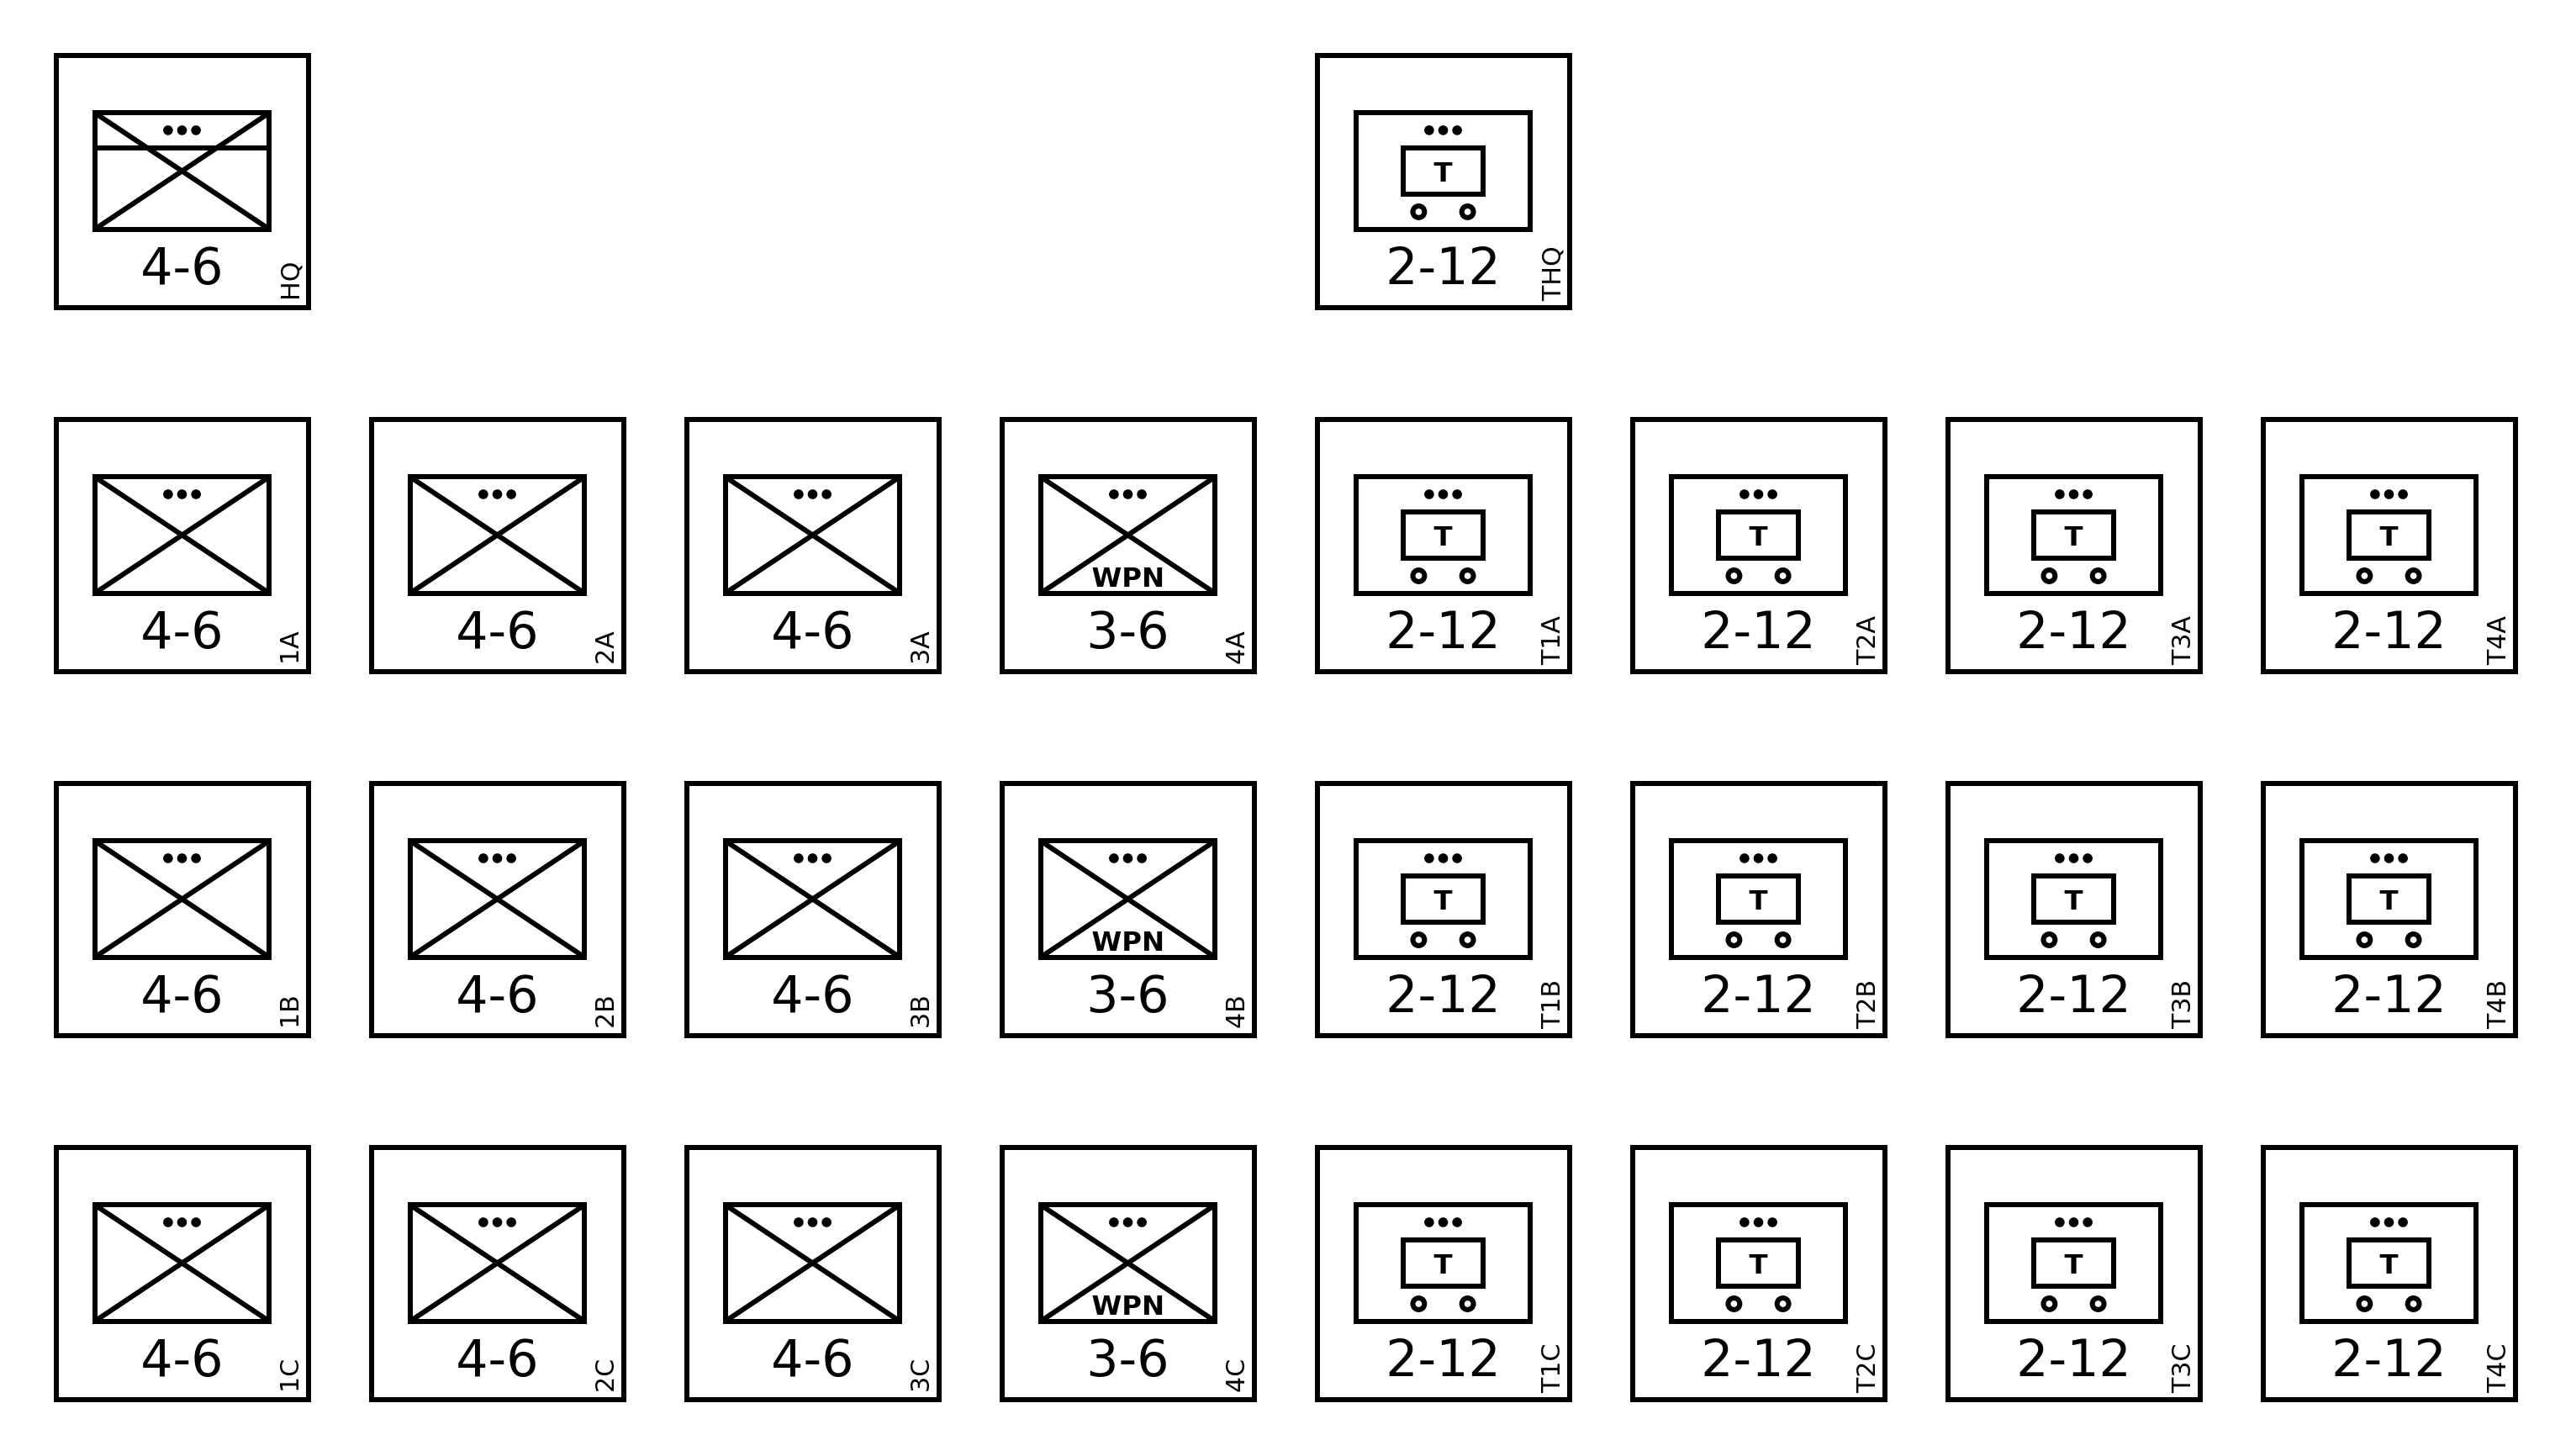
\includegraphics[width=\linewidth]{orders-of-battle/british-infantry-battalion-early-1960s.png}
\end{figure}

\begin{figure}[h]
    \subsection{Field Artillery Regiment} This regiment [battalion] has four batteries (A/B/C/D) each with six Cardinal (M44) self-propelled guns.

    
\includegraphics[width=\linewidth]{orders-of-battle/british-field-artillery-regiment-early-1960s.png}
\end{figure}

\begin{figure}[h]
    \subsection{Heavy Artillery Regiment} This regiment [battalion] has four batteries (A/B/C/D), two of each which have two Honest John launchers (and are treated as sections) and two of which have four towed 8-inch M1 guns.

    
\includegraphics[width=\linewidth]{orders-of-battle/british-heavy-artillery-regiment-early-1960s.png}
\end{figure}

\clearpage

\begin{itemize}

    \item Table~\ref{table:ob-two-para}: 2 Para Battalion at the 1982 Battle of Goose Green. At this time, the battalion had attached half a battery of 105~mm Light Guns from Alma Battery of 29 Commando Regiment, RA, a section of Blowpipes from 43rd Air Defence Battery, RA, and a Recce Troop of 59 Independent Commando Squadron, RE.

        \begin{table*}[p]
            \centering
            \caption{2 Para at Goose Green}
            \label{table:ob-two-para}
            \small
            \begin{tabularx}{0.9\linewidth}{LLL}
                \toprule
                Element&Game Ground Unit&Notes\\
                \midrule

                Battalion HQ
                &\binarymultiply{1}{infantry HQ platoon}\\

                A Company
                &\binarymultiply{3}{infantry platoon}\\

                B Company
                &\binarymultiply{3}{infantry platoon}\\

                C Company
                &\binarymultiply{2}{infantry platoon} &Patrol Company\\

                D Company
                &\binarymultiply{3}{infantry platoon}\\

                Support Company
                &\binarymultiply{1}{infantry mortar platoon}\\
                &\binarymultiply{1}{infantry weapons platoon}&GPMGs\\
                &\binarymultiply{1}{infantry weapons platoon}&MILANs\\
                &\binarymultiply{1}{infantry platoon}&Engineers\\

                Alma Battery
                &\binarymultiply{1}{towed artillery section}&Three 105-mm Light Guns\\

                Blowpipe Section
                &\binarymultiply{2}{infantry SAM squad -- Blowpipe}\\

                Engineers Troop
                &\binarymultiply{1}{infantry platoon}\\

                \bottomrule
            \end{tabularx}
        \end{table*}

    \item Table~\ref{table:ob-twelth-infantry}: 12th Infantry Regiment at the 1982 Battle of Goose Green, with attachments from the 25th Infantry Regiment, 4th Airborne Artillery Regiment, 601st Anti-Aircraft Artillery Group.

        \begin{table*}[p]
            \centering
            \caption{12IR at Goose Green}
            \label{table:ob-twelth-infantry}
            \small
            \begin{tabularx}{0.9\linewidth}{LLL}
                \toprule
                Element&Game Ground Unit&Notes\\
                \midrule
                Regimental HQ
                &\binarymultiply{1}{infantry HQ platoon}\\

                SAM Section
                &\binarymultiply{2}{infantry SAM squad -- SA-7B}\\

                A Company 12IR
                &\binarymultiply{5}{infantry platoon}\\

                B Company 12IR
                &\binarymultiply{3}{infantry platoon}\\

                C Company 25IR
                &\binarymultiply{2}{infantry platoon}\\
                &\binarymultiply{1}{infantry weapons platoon}\\

                C Company 12IR
                &\binarymultiply{2}{infantry platoon}\\
                &\binarymultiply{1}{infantry weapons platoon}\\

                A Battery, 4AAR
                &\binarymultiply{1}{towed artillery section}&Three 105-mm Pack Howitzers\\

                B Battery, 601 GADA
                &\binarymultiply{1}{Oerlikon 35~mm GDF section}&Two guns\\
                &\binarymultiply{1}{towed FCR-D}&Skyguard\\

                9th Engineering Company
                &\binarymultiply{1}{infantry platoon}\\

                \midrule

                3 Section B Battery 601AAAG
                &\binarymultiply{1}{Rh-202 20~mm battery}&Six guns\\
                &\binarymultiply{1}{EWR}&Elta\\

                Security Company
                &\binarymultiply{1}{infantry platoon}&\\

                \bottomrule
            \end{tabularx}
        \end{table*}

    \item Tables~\ref{table:ob-british-armored-regiment-early-1960s}, \ref{table:ob-british-apc-infantry-battalion-early-1960s}, \ref{table:ob-british-armored-regiment-early-1960s}, \ref{table:ob-british-infantry-battalion-early-1960s}, \ref{table:ob-british-field-artillery-regiment-early-1960s}, and \ref{table:ob-british-heavy-artillery-regiment-early-1960s}: An armored regiment, APC infantry battalion, infantry battalion, field artillery regiment, and heavy artillery regiment of the British Army from about 1960. In the British Army, regiments are battalion-level units.%

        \begin{table*}[p]

            \centering

            \caption{British Army Armored Regiment (Early 1960s)}
            \label{table:ob-british-armored-regiment-early-1960s}
            \small
            \begin{tabularx}{0.9\linewidth}{LLL}
                \toprule
                Element&Game Ground Unit&Notes\\
                \midrule
                \binarymultiply{1}{Regimental HQ}
                &\binarymultiply{1}{armored HQ platoon}\\

                \binarymultiply{1}{Reconnaissance Squadron}
                &\binarymultiply{3}{light reconnaissance/tank platoon}&\binarymultiply{15}{Ferret/Saladin}\\

                \binarymultiply{3}{Tank Squadrons} (A/B/C) each:
                &\binarymultiply{3}{medium tank platoon}&\binarymultiply{14}{Centurion}\\
                &\binarymultiply{1}{heavy tank platoon}&\binarymultiply{3}{Conqueror}\\

                \bottomrule
            \end{tabularx}

            \vspace{\floatsep}

            \caption{British Army APC Infantry Battalion (Early 1960s)}
            \label{table:ob-british-apc-infantry-battalion-early-1960s}
            \small
            \begin{tabularx}{0.9\linewidth}{LLL}
                \toprule
                Element&Game Ground Unit&Notes\\
                \midrule
                \binarymultiply{1}{Battalion HQ}
                &\binarymultiply{1}{armored HQ platoon}\\

                \binarymultiply{3}{Infantry Companies} (A/B/C) each:
                &\binarymultiply{3}{infantry platoon}&\\
                &\binarymultiply{1}{infantry weapons platoon}&\\
                &\binarymultiply{4}{light APC platoon}&\binarymultiply{17}{Saracen/FV432}\\

                \bottomrule
            \end{tabularx}

            \vspace{\floatsep}

            \caption{British Army Infantry Battalion (Early 1960s)}
            \label{table:ob-british-infantry-battalion-early-1960s}
            \small
            \begin{tabularx}{0.9\linewidth}{LLL}
                \toprule
                Element&Game Ground Unit&Notes\\
                \midrule
                \binarymultiply{1}{Battalion HQ}
                &\binarymultiply{1}{infantry HQ platoon}\\
                &\binarymultiply{1}{truck platoon}&\\

                \binarymultiply{4}{Infantry Companies} (A/B/C/D) each:
                &\binarymultiply{3}{infantry platoon}&\\
                &\binarymultiply{1}{infantry weapons platoon}&\\
                &\binarymultiply{4}{truck platoon}&\\

                \bottomrule
            \end{tabularx}

            \vspace{\floatsep}

            \caption{British Army Field Artillery Regiment (Early 1960s)}
            \label{table:ob-british-field-artillery-regiment-early-1960s}
            \small
            \begin{tabularx}{0.9\linewidth}{LLL}
                \toprule
                Element&Game Ground Unit&Notes\\
                \midrule
                \binarymultiply{1}{Regimental HQ}
                &\binarymultiply{1}{mobile HQ platoon}\\

                \binarymultiply{4}{Batteries} (A/B/C/D) each:
                &\binarymultiply{1}{tracked artillery battery}&\binarymultiply{6}{Cardinal (M44)}\\

                \bottomrule
            \end{tabularx}
        \end{table*}

        \begin{table*}[p]
            \centering
            \caption{British Army Heavy Artillery Regiment (Early 1960s)}
            \label{table:ob-british-heavy-artillery-regiment-early-1960s}
            \small
            \begin{tabularx}{0.9\linewidth}{LLL}
                \toprule
                Element&Game Ground Unit&Notes\\
                \midrule
                \binarymultiply{1}{Regimental HQ}
                &\binarymultiply{1}{mobile HQ platoon}\\

                \binarymultiply{2}{Batteries} (A/B) each:
                &\binarymultiply{1}{mobile rocket section}&\binarymultiply{2}{Honest John}\\

                \binarymultiply{2}{Batteries} (C/D) each:
                &\binarymultiply{1}{towed artillery battery}&\binarymultiply{4}{8-inch Gun M1}\\
                &\binarymultiply{1}{truck platoon}&\\

                \bottomrule
            \end{tabularx}
        \end{table*}

    \item Table~\ref{table:ob-british-armored-regiment-mid-1980s}: An armored regiment of the British Army from about 1985.

        \begin{table*}[p]
            \centering
            \caption{British Army Armored Regiment (Mid 1980s)}
            \label{table:ob-british-armored-regiment-mid-1980s}
            \small
            \begin{tabularx}{0.9\linewidth}{LLL}
                \toprule
                Element&Game Ground Unit&Notes\\
                \midrule
                \binarymultiply{1}{Regimental HQ}
                &\binarymultiply{1}{armored HQ platoon}\\

                \binarymultiply{1}{Reconnaissance Troop}
                &\binarymultiply{2}{light tank platoon}&\binarymultiply{8}{Scorpion}\\

                \binarymultiply{1}{ATGW Troop}
                &\binarymultiply{3}{light anti-tank platoon}&\binarymultiply{9}{FV438}\\

                \binarymultiply{3}{Tank Squadrons} (A/B/C) each:
                &\binarymultiply{4}{heavy tank platoon}&\binarymultiply{14}{Chieftain}\\

                \bottomrule
            \end{tabularx}
        \end{table*}

    \item Tables~\ref{table:ob-soviet-tank-battalion-1980s},
        \ref{table:ob-soviet-bmp-motor-rifle-battalion-1980s},
        \ref{table:ob-soviet-btr-motor-rifle-battalion-1980s},
        \ref{table:ob-soviet-self-propelled-artillery-battalion-1980s},
        \ref{table:ob-soviet-artillery-battalion-1980s},
        \ref{table:ob-soviet-tank-regiment-1980s},
        \ref{table:ob-soviet-bmp-motor-rifle-regiment-1980s},
        \ref{table:ob-soviet-btr-motor-rifle-regiment-1980s},
        \ref{table:ob-soviet-artillery-regiment-1980s},
        \ref{table:ob-soviet-sam-regiment-1980s},
        \ref{table:ob-soviet-reconnaissance-battalion-1980s},
        \ref{table:ob-soviet-anti-tank-battalion-1980s},
        \ref{table:ob-soviet-ssm-battalion-1980s}, and
        \ref{table:ob-soviet-motor-rifle-division-1980s}:
        A Soviet front-line motor-rifle division from the 1980s with its constituent regiments and battalions.\note{Soviet Units}{These are from US Army FM 100-2-3 from 1991.}
        In the Soviet Army, regiments are brigade-level units.

        \begin{table*}[p]
            \centering\footnotesize

            \caption{Soviet Tank Battalion (1980s)}
            \label{table:ob-soviet-tank-battalion-1980s}
            \begin{tabularx}{0.9\linewidth}{LLL}
                \toprule
                Element&Game Ground Unit&Notes\\
                \midrule
                \binarymultiply{1}{Battalion HQ}
                &\binarymultiply{1}{armored HQ platoon}\\

                \binarymultiply{3}{Tank Companies} each:
                &\binarymultiply{3}{heavy tank platoon}&\binarymultiply{12}{T-64/72/80}\\

                \bottomrule
            \end{tabularx}

            \vspace{\floatsep}

            \caption{Soviet BMP Motor Rifle Battalion (1980s)}
            \label{table:ob-soviet-bmp-motor-rifle-battalion-1980s}
            \begin{tabularx}{0.9\linewidth}{LLL}
                \toprule
                Element&Game Ground Unit&Notes\\
                \midrule
                \binarymultiply{1}{Battalion HQ}
                &\binarymultiply{1}{armored HQ platoon}\\

                \binarymultiply{1}{Mortar Battery}
                &\binarymultiply{1}{towed mortar platoon}&M1943 120~mm mortar\\
                &\binarymultiply{1}{truck platoon}&\\

                \binarymultiply{1}{Grenade Launcher Platoon}
                &\binarymultiply{1}{light IFV/APC platoon}&\binarymultiply{3}{BMP-1/2}\\
                &\binarymultiply{1}{infantry weapons platoon}&\binarymultiply{6}{AGS-17 grenade launchers}\\

                \binarymultiply{3}{Motor Rifle Companies} each:
                &\binarymultiply{4}{light IFV platoon}&\binarymultiply{12}{BMP-1/2}\\
                &\binarymultiply{3}{infantry platoon}&\\
                &\binarymultiply{1}{infantry weapons platoon}&\binarymultiply{6}{PKM machine guns}\\
                &\binarymultiply{3}{SA-7/14/16 squad}&\binarymultiply{3}{SA-7/14/16}\\

                \bottomrule
            \end{tabularx}

            \vspace{\floatsep}

            \caption{Soviet BTR Motor Rifle Battalion (1980s)}
            \label{table:ob-soviet-btr-motor-rifle-battalion-1980s}
            \begin{tabularx}{0.9\linewidth}{LLL}
                \toprule
                Element&Game Ground Unit&Notes\\
                \midrule
                \binarymultiply{1}{Battalion HQ}
                &\binarymultiply{1}{armored HQ platoon}\\

                \binarymultiply{1}{Mortar Battery}
                &\binarymultiply{2}{towed mortar platoon}&\binarymultiply{8}{M1943 mortar}\\
                &\binarymultiply{2}{truck platoon}&\\

                \binarymultiply{1}{Anti-Tank Platoon}
                &\binarymultiply{1}{light IFV/APC platoon}&\binarymultiply{5}{BTR-60/70}\\
                &\binarymultiply{1}{infantry weapons platoon}&\binarymultiply{2}{recoilless rifle} and \binarymultiply{4}{ATGM}\\

                \binarymultiply{1}{Grenade Launcher Platoon}
                &\binarymultiply{1}{light IFV/APC platoon}&\binarymultiply{3}{BTR-60/70}\\
                &\binarymultiply{1}{infantry weapons platoon}&\binarymultiply{6}{AGS-17 grenade launchers}\\

                \binarymultiply{3}{Motor Rifle Companies} each:
                &\binarymultiply{4}{light APC platoon}&\binarymultiply{12}{BTR-60/70}\\
                &\binarymultiply{3}{infantry platoon}&\\
                &\binarymultiply{1}{infantry weapons platoon}&\binarymultiply{3}{PKM machine gun} and \binarymultiply{3}{ATGM}\\
                &\binarymultiply{3}{SA-7/14/16 squad}&\binarymultiply{3}{SA-7/14/16}\\

                \bottomrule
            \end{tabularx}

            \vspace{\floatsep}

            \caption{Soviet Self-Propelled Artillery Battalion (1980s)}
            \label{table:ob-soviet-self-propelled-artillery-battalion-1980s}
            \begin{tabularx}{0.9\linewidth}{LLL}
                \toprule
                Element&Game Ground Unit&Notes\\
                \midrule
                \binarymultiply{1}{Battalion HQ}
                &\binarymultiply{1}{mobile HQ platoon}\\

                \binarymultiply{3}{Howitzer Battery} each
                &\binarymultiply{1}{towed artillery battery}&\binarymultiply{6}{122-mm 2S1 Gvozdika}\\

                \bottomrule
            \end{tabularx}

            \vspace{\floatsep}

            \caption{Soviet Artillery Battalion (1980s)}
            \label{table:ob-soviet-artillery-battalion-1980s}
            \begin{tabularx}{0.9\linewidth}{LLL}
                \toprule
                Element&Game Ground Unit&Notes\\
                \midrule
                \binarymultiply{1}{Battalion HQ}
                &\binarymultiply{1}{mobile HQ platoon}\\

                \binarymultiply{3}{Howitzer Battery} each
                &\binarymultiply{1}{towed artillery battery}&\binarymultiply{6}{122-mm D-30}\\
                &\binarymultiply{1}{truck platoon}&\\

                \bottomrule
            \end{tabularx}

        \end{table*}

        \begin{table*}[p]
            \centering\footnotesize

            \caption{Soviet Tank Regiment (1980s)}
            \label{table:ob-soviet-tank-regiment-1980s}
            \begin{tabularx}{0.9\linewidth}{LLL}
                \toprule
                Element&Game Ground Unit&Notes\\
                \midrule
                \binarymultiply{1}{Regimental HQ}
                &\binarymultiply{1}{armored HQ platoon}\\
                &\binarymultiply{3}{SA-7/14/16 squad}\\
                &\binarymultiply{3}{light truck squad}\\
                \binarymultiply{1}{Reconnaissance Company}
                &\binarymultiply{1}{light IFV platoon}&\binarymultiply{3}{BMP-1/2}\\
                &\binarymultiply{1}{light reconnaissance platoon}&\binarymultiply{4}{BRDM-2}\\
                \binarymultiply{1}{Air-Defense Battery}
                &\binarymultiply{2}{SA-9/13 section}&\binarymultiply{4}{SA-9/13}\\
                &\binarymultiply{2}{ZSU-23-4 section}&\binarymultiply{4}{ZSU-23-4}\\
                \binarymultiply{3}{Tank Battalion}\\
                \binarymultiply{1}{Self-Propelled Artillery Battalion}\\
                \bottomrule
            \end{tabularx}

            \vspace{\floatsep}

            \caption{Soviet BMP Motor-Rifle Regiment (1980s)}
            \label{table:ob-soviet-bmp-motor-rifle-regiment-1980s}
            \begin{tabularx}{0.9\linewidth}{LLL}
                \toprule
                Element&Game Ground Unit&Notes\\
                \midrule
                \binarymultiply{1}{Regimental HQ}
                &\binarymultiply{1}{armored HQ platoon}\\
                &\binarymultiply{3}{SA-7/14/16 squad}\\
                &\binarymultiply{3}{light truck squad}\\
                \binarymultiply{1}{Reconnaissance Company}
                &\binarymultiply{1}{light IFV platoon}&\binarymultiply{3}{BMP-1/2}\\
                &\binarymultiply{1}{light reconnaissance platoon}&\binarymultiply{4}{BRDM-2}\\
                \binarymultiply{1}{Anti-Tank Battery}
                &\binarymultiply{3}{light anti-tank platoon}&\binarymultiply{9}{BRDM-2 ATGM}\\
                \binarymultiply{1}{Air-Defense Battery}
                &\binarymultiply{2}{SA-9/13 section}&\binarymultiply{4}{SA-9/13}\\
                &\binarymultiply{2}{ZSU-23-4 section}&\binarymultiply{4}{ZSU-23-4}\\
                \binarymultiply{3}{BMP Motor-Rifle Battalions}\\
                \binarymultiply{1}{Tank Battalion}\\
                \binarymultiply{1}{Self-Propelled Artillery Battalion}\\
                \bottomrule
            \end{tabularx}

            \vspace{\floatsep}

            \caption{Soviet BTR Motor-Rifle Regiment (1980s)}
            \label{table:ob-soviet-btr-motor-rifle-regiment-1980s}
            \begin{tabularx}{0.9\linewidth}{LLL}
                \toprule
                Element&Game Ground Unit&Notes\\
                \midrule
                \binarymultiply{1}{Regimental HQ}
                &\binarymultiply{1}{armored HQ platoon}\\
                &\binarymultiply{3}{SA-7/14/16 squad}\\
                &\binarymultiply{3}{light truck squad}\\
                \binarymultiply{1}{Reconnaissance Company}
                &\binarymultiply{1}{light IFV platoon}&\binarymultiply{3}{BMP-1/2}\\
                &\binarymultiply{1}{light reconnaissance platoon}&\binarymultiply{4}{BRDM-2}\\
                \binarymultiply{1}{Anti-Tank Battery}
                &\binarymultiply{3}{light anti-tank platoon}&\binarymultiply{9}{BRDM-2 ATGM}\\
                \binarymultiply{1}{Air-Defense Battery}
                &\binarymultiply{2}{SA-9/13 section}&\binarymultiply{4}{SA-9/13}\\
                &\binarymultiply{2}{ZSU-23-4 section}&\binarymultiply{4}{ZSU-23-4}\\
                \binarymultiply{3}{BTR Motor-Rifle Battalions}\\
                \binarymultiply{1}{Tank Battalion}\\
                \binarymultiply{1}{Artillery Battalion}\\
                \bottomrule
            \end{tabularx}

        \end{table*}

        \begin{table*}[p]
            \centering\footnotesize

            \caption{Soviet Artillery Regiment (1980s)}
            \label{table:ob-soviet-artillery-regiment-1980s}
            \begin{tabularx}{0.9\linewidth}{LLL}
                \toprule
                Element&Game Ground Unit&Notes\\
                \midrule
                \binarymultiply{1}{Regimental HQ}
                &\binarymultiply{1}{armored HQ platoon}\\
                \binarymultiply{3}{Self-Propelled Artillery Battalions each}
                &\binarymultiply{3}{light armored artillery battery}&\binarymultiply{18}{152-mm 2S3}\\
                \binarymultiply{1}{Rocket Artillery Battalion}
                &\binarymultiply{3}{mobile rocket artillery battery}&\binarymultiply{18}{BM-21}\\
                \bottomrule
            \end{tabularx}

            \vspace{\floatsep}

            \caption{Soviet SAM Regiment (1980s)}
            \label{table:ob-soviet-sam-regiment-1980s}
            \begin{tabularx}{0.9\linewidth}{LLL}
                \toprule
                Element&Game Ground Unit&Notes\\
                \midrule
                \binarymultiply{1}{Regimental HQ}
                &\binarymultiply{1}{armored HQ platoon}\\
                &\binarymultiply{3}{SA-7/14/16 squad}\\
                &\binarymultiply{3}{light truck squad}\\
                \binarymultiply{1}{EWR Battery}
                &\binarymultiply{2}{EWR-B}&\binarymultiply{2}{Long Track EWR} and \binarymultiply{1}{Thin Skin HFR}\\
                \binarymultiply{5}{SAM Batteries each}
                &\binarymultiply{1}{SA-6 battery}&\binarymultiply{4}{SA-6 TELAR} and \binarymultiply{1}{Straight Flush TTR}\\
                &\binarymultiply{1}{SA-7/14/16 squad}\\
                &\binarymultiply{1}{light truck squad}\\
                \bottomrule
            \end{tabularx}

            \vspace{\floatsep}

            \caption{Soviet Reconnaissance Battalion (1980s)}
            \label{table:ob-soviet-reconnaissance-battalion-1980s}
            \begin{tabularx}{0.9\linewidth}{LLL}
                \toprule
                Element&Game Ground Unit&Notes\\
                \midrule
                \binarymultiply{1}{Battalion HQ}
                &\binarymultiply{1}{armored HQ platoon}\\
                \binarymultiply{2}{Reconnaissance Company} each
                &\binarymultiply{2}{light IFV platoon}&\binarymultiply{6}{BMP-1/2}\\
                &\binarymultiply{2}{infantry platoon}\\
                &\binarymultiply{1}{heavy tank platoon}&\binarymultiply{3}{T-64/72/80}\\
                \binarymultiply{1}{Reconnaissance Assault Company}
                &\binarymultiply{3}{light reconnaissance platoon}&\binarymultiply{18}{BRDM-2}\\
                \bottomrule
            \end{tabularx}

            \vspace{\floatsep}

            \caption{Soviet Anti-Tank Battalion (1980s)}
            \label{table:ob-soviet-anti-tank-battalion-1980s}
            \begin{tabularx}{0.9\linewidth}{LLL}
                \toprule
                Element&Game Ground Unit&Notes\\
                \midrule
                \binarymultiply{1}{Battalion HQ}
                &\binarymultiply{1}{armored HQ platoon}\\
                \binarymultiply{2}{Anti-Tank Gun Battery} each
                &\binarymultiply{1}{towed anti-tank battery}&\binarymultiply{6}{100-mm MT-12}\\
                &\binarymultiply{1}{light APC platoon}&\binarymultiply{7}{MT-LB}\\
                \binarymultiply{1}{ATGM Battery}
                &\binarymultiply{3}{light anti-tank platoon}&\binarymultiply{9}{BRDM-2 ATGM}\\
                \bottomrule
            \end{tabularx}

            \vspace{\floatsep}

            \caption{Soviet SSM Battalion (1980s)}
            \label{table:ob-soviet-ssm-battalion-1980s}
            \begin{tabularx}{0.9\linewidth}{LLL}
                \toprule
                Element&Game Ground Unit&Notes\\
                \midrule
                \binarymultiply{1}{Battalion HQ}
                &\binarymultiply{1}{mobile HQ platoon}\\
                \binarymultiply{2}{SSM Battery} each
                &\binarymultiply{1}{mobile missile artillery section}&\binarymultiply{2}{FROG-7 or SS-21}\\
                \bottomrule
            \end{tabularx}

        \end{table*}

        \clearpage

        \begin{table*}[p]
            \centering\footnotesize

            \caption{Soviet Motor-Rifle Division (1980s)}
            \label{table:ob-soviet-motor-rifle-division-1980s}
            \begin{tabularx}{0.9\linewidth}{LLL}
                \toprule
                Element&Game Ground Unit&Notes\\
                \midrule
                \binarymultiply{1}{Divisional HQ}
                &\binarymultiply{1}{armored HQ platoon}\\
                &\binarymultiply{6}{SA-7/14/16 squad}\\
                &\binarymultiply{6}{light truck squad}\\

                \binarymultiply{1}{Reconnaissance Battalion}\\
                \binarymultiply{1}{Anti-Tank Battalion}\\
                \binarymultiply{1}{SSM Battalion}\\

                \binarymultiply{1}{BMP Motor-Rifle Regiment}\\
                \binarymultiply{2}{BTR Motor-Rifle Regiment}\\
                \binarymultiply{1}{Tank Regiment}\\
                \binarymultiply{1}{Artillery Regiment}\\
                \binarymultiply{1}{SAM Regiment}\\
                \bottomrule
            \end{tabularx}

        \end{table*}

\end{itemize}
